 \documentclass{report}
 
\usepackage[utf8]{inputenc} 
\usepackage[T1]{fontenc}      
\usepackage[top=3.5cm, bottom=3cm, left=4.0cm, right=4.0cm]{geometry}
\usepackage{graphicx}
\graphicspath{{figures/}{../figures}}

\begin{document}

\chapter{Association en cascade, AO en régime linéaire et saturé}


\section*{Exercice 2}
On suppose d'abord que $R_{s}=0$ et $R_{e}=\infty$, et on suppose que le cadre en pointillés représente un quadripôle tel que : $V_{s}=GV_{e}$. Trouvez  une équation différentielle en $i(t)$.

Quel est la condition sur $G$ pour voir apparaître des oscillations sinusoïdales pures ? Donnez les valeurs les valeurs de $G$ et de $f_{0}$ la fréquence de ces oscillations.

Comment cette condition change lorsque $R_{s}\neq 0$ et $R_{e}\neq\infty$?
\begin{figure}[!h]
\centering
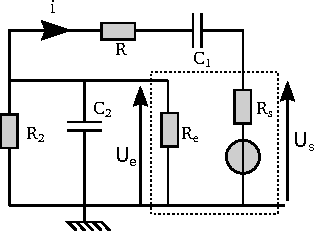
\includegraphics[width=0.5\linewidth]{circuit_5.pdf}
\end{figure}

\newpage

\section*{Question de cours}
Donnez le schéma de montage d'un \textbf{intégrateur} en précisant la fonction de transfert.
\section*{Exercice 5}
On suppose l'AO idéal : déterminez $U_{-}(t)$ et $U_{s}(t)$. \textit{Indication : Remarquez qu'il y a une rétroaction sur la borne $+$}.
\begin{figure}[!h]
\centering
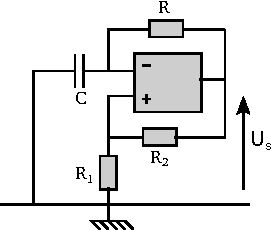
\includegraphics[width=0.5\linewidth]{circuit_3.pdf}
\end{figure}
\section*{Question supplémentaire}
Comment réaliser un générateur de courant idéal?

\newpage

\section*{Question de cours}

Quel est le lien entre la fonction de transfert d'un quadripôle et l'équation différentielle sur la tension d'entrée et de sortie?
\section*{Exercice}
Après avoir précisé le comportement du circuit en basse et haute fréquence, déterminez la fonction de transfert de ce filtre sous la forme canonique. Quel est le rôle de ce filtre? Tracez le diagramme de Bode correspondant.
\begin{figure}[!h]
\centering
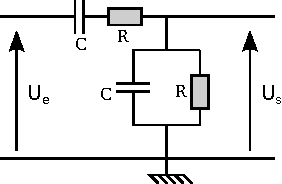
\includegraphics[width=0.5\linewidth]{circuit_1.pdf}
\end{figure}

\section*{Question supplémentaire}

On réalise ce montage. Pour quelles valeurs de $R1$ et $R2$ voit-on apparaître des oscillations sur $U_{e}$?
\begin{figure}[!h]
\centering
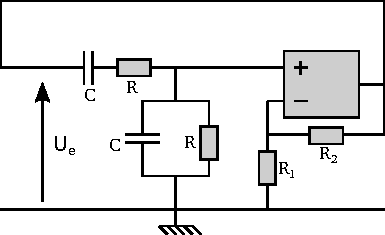
\includegraphics[width=0.6\linewidth]{circuit_4.pdf}
\end{figure}

\newpage

\section*{Question de cours}
Quel est le lien entre la fonction de transfert d'un quadripôle et l'équation différentielle sur la tension d'entrée et de sortie?
\section*{Exercice 6}
Après avoir précisé le comportement du circuit en basse et haute fréquence, déterminez la fonction de transfert de ce filtre sous la forme canonique.
\textit{Indication : on s'évertuera à la mettre sous la forme suivante, en précisant les expressions de a, b etc ainsi que leurs dimensions : 
\begin{equation}
\underline{H}(j\omega)=\frac{1}{a+\frac{1}{bj\omega}+cj\omega}
\end{equation}
}
\begin{figure}[!h]
\centering
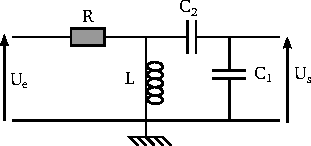
\includegraphics[width=0.4\linewidth]{circuit_7.pdf}
\end{figure}

On envisage désormais le montage suivant : 
\begin{figure}[!h]
\centering
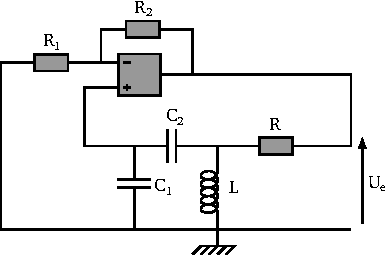
\includegraphics[width=0.4\linewidth]{circuit_8.pdf}
\end{figure}

A quelle condition a t-on des oscillations sur le circuit?

\section*{Exercice supplémentaire}
Est-il possible d'avoir des oscillations sur un tel circuit si H est un passe-bas d'ordre 2? A quelles conditions? 
Même questions pour un passe haut d'ordre 2.
\begin{figure}[!h]
\centering
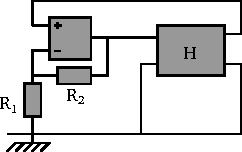
\includegraphics[width=0.3\linewidth]{circuit_9.pdf}
\end{figure}

\newpage

\section*{Remplissage d'un réservoir d'hélium}
\subsection*{Première version}
On considère ici un système de remplissage d'un réservoir d'hélium. Par évaporation, de l'hélium s'échappe constamment du réservoir. Pour des raisons pratiques, on souhaite maintenir le niveau d'He à un niveau minimum $h_{min}$.

Pour cela, une vanne (V) introduit de l'hélium dès que la tension à ses bornes est positive. Pour mesurer le niveau d'He, un transducteur (T) fournit une tension $e$ proportionnelle à la hauteur d'He : $e= \alpha h$. (P) est un potentiomètre dont la résistance varie de $0$ à $800\Omega$.

\textit{Données : $R_{1} = 100k\Omega$, $R_{2}=R{3}=200\Omega$, $\alpha = 5V/m$. L'AO est supposé idéal.}

\begin{figure}[!h]
\centering
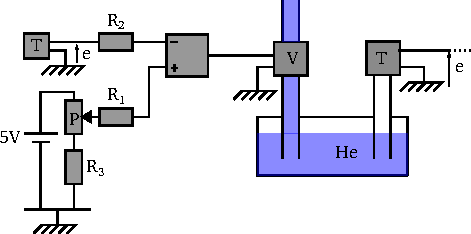
\includegraphics[width=0.8\linewidth]{circuit_10.pdf}
\end{figure}

Comment fonctionne ce montage? Donnez la hauteur minimale $h_{min}$ et maximale $h_{max}$. Quel est le défaut de ce système?

\subsection*{Seconde version}
On introduit une rétroaction sur l'AO avec une résistance.

\begin{figure}[!h]
\centering
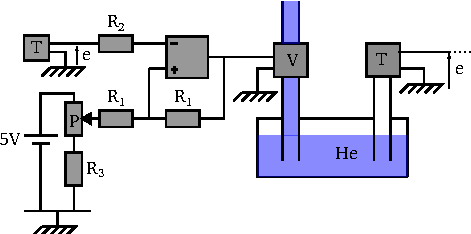
\includegraphics[width=0.8\linewidth]{circuit_11.pdf}
\end{figure}

Comment fonctionne ce nouveau montage? Quel est son intérêt? Donnez la hauteur minimale $h_{min}$ et maximale $h_{max}$.

\end{document}
